\section{BAYESIAN OPTIMIZATION}

\begin{yellowbox}{\textbf{NOMENCLATURE}}
    \begin{tabularx}{\columnwidth}{ll}
        $\sigma_t^2(x)$ & Posterior variance\\
        \addlinespace[2pt]
        $$ & \\
        $$ & \\
        $$ & \\
        $$ & \\
        $$ & \\
        $$ & \\
        $$ & \\
        $$ & \\
   
    \end{tabularx}
\end{yellowbox}

\begin{whitebox}{\textbf{BAYESIAN OPTIMIZATION (BO)}}
    \begin{itemize}
        \item Goal: find global optimum of an unknown function $f^*$ in a sample-efficient manner i.e. with as few queries as possible
        \begin{align*}
            x^*\in\arg\max_{x\in\mathcal{X}}f^*(x)
        \end{align*}
        \item Background: it is costly to obtain observations (evaluate a model) e.g. to evaluate the predictive performance after training a neural network
        \item Observation model
        \begin{align*}
            y_t=f^*(x_t)+\epsilon_t
        \end{align*}
        where we use a surrogate $f$ (e.g. GP) for the objective function $f^*$ and have noise $\epsilon_t$
        \item Bandit policy/acquisition function: how to sequentially query in order to achieve the goal?
        \begin{itemize}
            \item Exploration-exploitation tradeoff
            \item Cumulative regret
            \begin{align*}
                R_T=\sum_{t\leq T}f^*(x^*)-f^*(x_t)
            \end{align*}
        \end{itemize}
        \begin{itemize}
            \item Sublinearity: $\frac{R_{(T)}}{T}\to 0$
        \end{itemize}
    \end{itemize}
\end{whitebox}

\begin{whitebox}{\textbf{ASSUMPTIONS}}
    \begin{itemize}
        \item Domain
        \begin{itemize}
            \item $|\mathcal{X}|<\infty$ or $\mathcal{X}\subseteq\mathbb{R}^d$ is compact
        \end{itemize}
        \item Noise
        \begin{itemize}
            \item $\epsilon_t\sim\mathrm{subG}$ (sub-Gaussian) zero-mean i.i.d.
        \end{itemize}
        \item Objective/reward function
        \begin{itemize}
            \item $f^*\sim\mathrm{GP}(0,k)$ (sample path from a GP)
            \item $f^*\in\mathcal{H}_k$ (reproducing kernel Hilbert space RKHS)
            \item $f^*:\mathcal{X}\to\mathbb{R}$
        \end{itemize}
    \end{itemize}
\end{whitebox}

\begin{whitebox}{\textbf{OPTIMISTIC POLICIES}}
    \begin{itemize}
        \item Probability of improvement
        \begin{align*}
            \mathrm{PI}(x)=P(f^*(x)>y_t^*\mid\mathrm{history}_{1:t})=\Phi\left(\frac{\mu(t)-y^*_t}{\sigma_t(x)}\right)
        \end{align*}
        where $P(f^*\mid\mathrm{history})\sim\mathrm{GP}(\mu_t,\sigma_t)$
        \begin{itemize}
            \item Note: $\sigma_t(x)\downarrow\implies\mathrm{PI}\uparrow$ meaning it is incentivized that we pick points close to previous maximas (there $\sigma_t$ is small) which have posterior mean larger than the best previously observerd point
            \item May not explore sufficiently!
        \end{itemize}
        \item Expected improvement
        \begin{align*}
            \mathrm{EI}(x)=\mathbb{E}((f^*(x)-y_t^*)_+\mid\mathrm{history}_{1:t})
        \end{align*}
        \begin{itemize}
            \item Unknown reward conditioned on history (argument of $\mathbb{E}$ above) is sample from posterior GP distribution, so there exists a closed form expression for the expectation in terms of $\mu_t,\sigma_t$
            \item $\mathrm{EI}$ looks at probability as well as magnitude of improvement
            \item $\mathrm{EI}$ is good practical choice of policy
        \end{itemize}
        \item Other optimistic policies (acquisition functions)
        \begin{itemize}
            \item Thompson sampling
            \item Upper confidence bound (UCB)
        \end{itemize}
    \end{itemize}
    \begin{center}
    \resizebox{0.95\linewidth}{!}{
        \includegraphics[
        page=11,
        trim = {2.0cm, 1.0cm, 1.5cm, 3.7cm}, % left, bottom, right, top
        clip
        ]{media/22HS_Tut08_BO.pdf}
    }
    \end{center}
\end{whitebox}

\begin{whitebox}{\textbf{EXPLORATION AND EXPLOITATION}}
    \begin{itemize}
        \item Exploration guided by the confidence sets/bounds
        \begin{align*}
            \mathcal{C}_t(x)=[\mu_t(x)-\beta_t\sigma_t(x),\mu_t(x)+\beta_t\sigma_t(x)]
        \end{align*}
        used as a proxy for the unknown reward $f^*(t)$ at every time $t$
        \begin{itemize}
            \item Width $\longleftrightarrow$ current uncertainty
            \item Center $\longleftrightarrow$ current knowledge
        \end{itemize}
        \item Theorem: if $f^*\sim\mathrm{GP}(0,k)$, then for a certain choice of $\beta_t$, the confidence sets are any-time valid with high probability, i.e.
        \begin{align*}
            P(f^*(x)\in\mathcal{C}_{t-1}(x),\ \forall x\in\mathcal{X},t\geq 1)\geq 1-\delta,\quad\delta\in(0,1)
        \end{align*}
        \begin{itemize}
            \item By using $\mathcal{C}_t$ instead of the unknown reward, the single-step regret will be controlled by the width of the set, whp (with high probability)
        \end{itemize}
    \end{itemize}
\end{whitebox}

\begin{whitebox}{\textbf{WORST CASE REGRET WITH UCB}}
    \begin{itemize}
        \item Whp, $\mathcal{C}_t$ gives
        \begin{align*}
            &|f(\mathbf{x}_t)-\mu_{t-1}(\bm{x}_t)|\leq\beta_t\sigma_{t-1}(\bm{x}_t)\\
            &|f(\mathbf{x}^*)-\mu_{t-1}(\bm{x}^*)|\leq\beta_t\sigma_{t-1}(\bm{x}^*)
        \end{align*}
        Use the UCB to obtain the regret
        \begin{align*}
            r_t=f(\bm{x}^*)-f(\bm{x}_t)&\leq\mu_{t-1}(\bm{x}^*)+\beta_t\sigma_{t-1}(\bm{x}^*)-f(\bm{x}_t)\\
            &\leq\mu_{t-1}(\bm{x}_t)+\beta_t\sigma_{t-1}(\bm{x}_t)-f(\bm{x}_t)\\
            &\leq 2\beta_t\sigma_{t-1}(\bm{x}_t)
        \end{align*}
        Invoke the confidence bound $T$ times, with a special choice of $\beta_t$
        \begin{align*}
            R_T&=\sqrt{\sum_{i=1}^Tr_t}\\
            &\text{using Cauchy-Schwarz}\\
            &\leq\sqrt{T}\sqrt{\sum_{i=1}^Tr_t^2}\\
            &\leq\sqrt{T}\sqrt{\sum_{i=1}^T4\beta_t^2\sigma_{t-1}^2(\bm{x}_t)}\\
            &\text{since $\beta_t$ is non-decreasing}\\
            &\leq\sqrt{T}\sqrt{4\beta_T^2\sum_{i=1}^T\sigma_{t-1}^2(\bm{x}_t)}\\
            &\leq\mathcal{O}\left(\beta_T\sqrt{T\gamma_T}\right)\\
            &=\tilde{\mathcal{O}}\left(\sqrt{T\gamma_T}\right),\quad\beta_T=B+\sigma_n^2\sqrt{2\gamma_T+2\log\left(\sfrac{1}{\delta}\right)}\\
            &\text{where $\tilde{\mathcal{O}}$ omits log factors}
        \end{align*}
        \item Sublinearity
        \begin{align*}
            R_T=\mathcal{O}(T^\alpha),\quad\alpha<1
        \end{align*}
    \end{itemize}
\end{whitebox}

\begin{itemize}
    \item Largest reward seen up to now
    \begin{align*}
        y_t^*=\arg\max_{i\leq t}y_i
    \end{align*}
\end{itemize}

\begin{whitebox}{\textbf{THOMPSON SAMPLING}}
    \begin{align*}
        x_{t+1}\in\arg\max_x \tilde{f}(x)
    \end{align*}
    where $\tilde{f}\sim p(f|H_t)$ is a sample path from the GP posterior (based on data $H_t=\{(x_i,y_i)\}_{i\leq t}$)
    \begin{itemize}
        \item 
    \end{itemize}
\end{whitebox}

\begin{whitebox}{\textbf{UPPER CONFIDENCE BOUND (UCB)}}
    \begin{align*}
        x_{t+1}\in\arg\max_x \underbrace{\mu_t(x)+\beta_t\sigma_t(x)}_{\text{UCB}}
    \end{align*}
    \begin{itemize}
        \item Optimistic bandit policy i.e. we are maximizing some statistical upper-bound on the reward
        \item More practical than Thompson sampling
        \item $\beta_t$ should be non-decreasing as posterior variance $\sigma_t$ naturally decreases
        \item $\beta_t\uparrow$ incentivises exploration
        \item Algorithm
        \begin{center}
            \begin{algorithmic}
                \Require $\beta_t$
                % \Loop
                \For{$t\in\{1,\dots,T\}$}
                %\Comment{TODO}
                \State Estimate $\mu_{t-1},\sigma_{t-1}$ using $(x_i,y_i)_{i<t}$
                \State Choose $x_t=\arg\max_{x\in\mathcal{X}}\mu_{t-1}(x)+\beta_t\sigma_{t-1}(x)$
                \State Observe $y_t$
                \EndFor
                % \EndLoop
            \end{algorithmic}
        \end{center}
    \end{itemize}
\end{whitebox}

\begin{whitebox}{\textbf{OTHER POLICIES}}
    \begin{itemize}
        \item Linear reward
        \begin{align*}
            f^*(x)=x^\top w^*,\quad x\in\mathbb{R}^d
        \end{align*}
        \item Greedy policy
        \begin{itemize}
            \item Pick first action uniformly at random and observe $y_1$
            \item No exploration/exploitation principle
            \item Non i.i.d. because $x_t$ depends on $\hat{w}$ (and thus history $(x_i,y_i)_{i<t}$
            \item Algorithm
            \begin{algorithmic}
                \footnotesize
                % \Loop
                \For{$t\in\{2,\dots,T\}$}
                %\Comment{TODO}
                \State Estimate $\hat{w}_{t-1}$ using $(x_i,y_i)_{i<t}$
                \State Choose $x_t=\arg\max_{x\in\mathcal{X}}x^\top\hat{w}_{t-1}$ (ignores noise)
                \State Observe $y_t$
                \EndFor
                % \EndLoop
            \end{algorithmic}
        \end{itemize}
        \item Explore-then-commit policy
        \begin{itemize}
            \item Algorithm
            \begin{algorithmic}
                \footnotesize
                \Require $T_0$
                % \Loop
                \For{$t\in\{1,\dots,T_0\}$}
                %\Comment{TODO}
                \State Choose $x_t$ uniformly at random
                \Comment{Collect i.i.d. data set}
                \State Observe $y_t$
                \EndFor
                % \EndLoop
                \State Esimate $\hat{w}$ using $(x_t,y_t)_{t\leq T_0}$
                % \Loop
                \For{$t\in\{T_0,\dots,T\}$}
                \State Choose $x_t=\arg\max_{x\in\mathcal{X}}x^\top\hat{w}$
                \Comment{Keep taking the same action!}
                \State Observe $y_t$                
                \EndFor
                % \EndLoop
            \end{algorithmic}
        \end{itemize}
    \end{itemize}
\end{whitebox}

\begin{whitebox}{\textbf{INFORMATION GAIN}}
    \begin{align*}
        I(\bm{y}_T;\bm{f}_T)&=H(\bm{y}_T)-H(\bm{y}_T\mid \bm{f}_T)\\
        &=\frac{1}{2}\log\det(\mathbb{I}+\sigma^{-2}K_T)\\
        &\text{Use Hadamard's inequality for PSD matrices}\\
        &\leq\frac{1}{2\sigma^2}\sum_{i\leq T}\lambda_i(K_T)
    \end{align*}
    where $\lambda_i$ are the eigenvalues of the kernel matrix $K_T$ (which depends on the data $x_1$ to $x_T$)
    \begin{itemize}
        \item Notion of learning complexity (what we learn about $f$ through a vector of noisy observations $y$)
        \item Assumptions
        \begin{itemize}
            \item GP model
            \item Sub-Gaussian i.i.d. noise
        \end{itemize}
        \item Rewrite in terms of posterior variance $\sigma_t^2(x)$ using entropy chain-rule
        \begin{align*}
            I(\bm{y}_T;\bm{f}_T)=\frac{1}{2}\sum_{t\leq T}\log\left(1+\frac{\sigma_t^2(x)}{\sigma_n^2}\right)
        \end{align*}
        \begin{itemize}
            \item Lemma
            \mathbox{
                \sum_{t\leq T}\sigma_t^2(x)\leq C\cdot I(\bm{y}_T;\bm{f}_T)\leq C\cdot\gamma_T
            }
            by using $s_t\leq C_1\log(1+s_t)$ where $s_t:=\frac{\sigma_t^2(x)}{\sigma_n^2}\in[0,M]$ assuming $s_0\in[0,M]$
        \end{itemize}
        \item Can obtain \textit{data-independent} bound via eigen-spectrum of the kernel operator
        \item Hardness of sequential learning comes from
        \begin{itemize}
            \item Complexity of estimating the unknown function
            \item Complexity of choosing the next action
        \end{itemize}
        \item Note: for i.i.d. Gaussian noise, the information gain $I$ does not depend on the function evaluations, therefore there might be better choices for an online measure of complexity
        \item $I$ appears naturally in more or less all worst-case regret bounds
        \item Noise level limits information gain at any time
    \end{itemize}
\end{whitebox}

\begin{whitebox}{\textbf{KERNEL FUNCTIONS}}
    \begin{itemize}
        \item For complex (e.g. non-differentiable) reward function, the GP assumption requires a rougher kernel
        \item The more complex the kernel, the more faster the information gain grows with $T$ and the slower the eigenvalues $\lambda_i$ of the kernel function (as more eigenfunctions are necessary to explain the kernel)
        \begin{itemize}
            \item Matérn
            \begin{align*}
                \lambda_k=\mathcal{O}(k^{-\frac{1+2\nu}{d}}),\quad \nu>\frac{1}{2}
            \end{align*}
            \item RBF
            \begin{align*}
                \lambda_k=\mathcal{O}(\exp(-k^{\frac{1}{d}}))
            \end{align*}
            with input dimension $d$
            \begin{center}
                \resizebox{0.90\linewidth}{!}{
                    \includegraphics[
                    page=19,
                    trim = {12.5cm, 1.0cm, 1.5cm, 9.5cm}, % left, bottom, right, top
                    clip
                    ]{media/22HS_Tut08_BO.pdf}
                }
            \end{center}
        \end{itemize}
        \item The performance of the algorithm highly depends on the kernel function
        \begin{itemize}
            \item Worst-case regret
            \begin{align*}
                R_T=\mathcal{O}(\sqrt{T\gamma_T}),\quad\gamma_T=\mathcal{O}(T^\alpha)
            \end{align*}
            \begin{itemize}
                \item While $R_T$ may still be sublinear for complex kernels, the rate with $T$ naturally gets worse (since the problem becomes harder in the worst case)
                \begin{center}
                    \resizebox{0.90\linewidth}{!}{
                        \includegraphics[
                        page=20,
                        trim = {11.3cm, 5.0cm, 2.35cm, 4.8cm}, % left, bottom, right, top
                        clip
                        ]{media/22HS_Tut08_BO.pdf}
                    }
                \end{center}
                \item Note: this is just a worst case guarantee, so it does not necessarily imply that the algorithm will always do worse (average case will be smoother than the worst case sample)
            \end{itemize}
            \item Choice of good kernel is difficult
            \begin{itemize}
                \item Overly complex kernel
                \begin{itemize}
                    \item Increases epistemic uncertainty of model
                    \item Posterior variance will be too large (confidence sets too wide), increasing our worst case regret
                    \begin{align*}
                        r_t=f(\bm{x}^*)-f(\bm{x}_t)\leq 2\beta_t\sigma_{t-1}(\bm{x}_t)
                    \end{align*}
                    using the UCB confidence set set $\mathcal{C}_t$
                \end{itemize}
                \item Overly simple kernel
                \begin{itemize}
                    \item The assumption $f^*\sim\mathrm{GP}(0,k)$ no longer holds, so the above worst case regret inequality does not hold i.e. anything could happen!
                \end{itemize}
                \begin{center}
                    \resizebox{0.95\linewidth}{!}{
                        \includegraphics[
                        page=21,
                        trim = {2.5cm, 2.0cm, 1.0cm, 9.0cm}, % left, bottom, right, top
                        clip
                        ]{media/22HS_Tut08_BO.pdf}
                    }
                \end{center}
            \end{itemize}
        \end{itemize}
    \end{itemize}
\end{whitebox}